\documentclass[twoside]{book}

% Packages required by doxygen
\usepackage{fixltx2e}
\usepackage{calc}
\usepackage{doxygen}
\usepackage[export]{adjustbox} % also loads graphicx
\usepackage{graphicx}
\usepackage[utf8]{inputenc}
\usepackage{makeidx}
\usepackage{multicol}
\usepackage{multirow}
\PassOptionsToPackage{warn}{textcomp}
\usepackage{textcomp}
\usepackage[nointegrals]{wasysym}
\usepackage[table]{xcolor}

% Font selection
\usepackage[T1]{fontenc}
\usepackage[scaled=.90]{helvet}
\usepackage{courier}
\usepackage{amssymb}
\usepackage{sectsty}
\renewcommand{\familydefault}{\sfdefault}
\allsectionsfont{%
  \fontseries{bc}\selectfont%
  \color{darkgray}%
}
\renewcommand{\DoxyLabelFont}{%
  \fontseries{bc}\selectfont%
  \color{darkgray}%
}
\newcommand{\+}{\discretionary{\mbox{\scriptsize$\hookleftarrow$}}{}{}}

% Page & text layout
\usepackage{geometry}
\geometry{%
  a4paper,%
  top=2.5cm,%
  bottom=2.5cm,%
  left=2.5cm,%
  right=2.5cm%
}
\tolerance=750
\hfuzz=15pt
\hbadness=750
\setlength{\emergencystretch}{15pt}
\setlength{\parindent}{0cm}
\setlength{\parskip}{3ex plus 2ex minus 2ex}
\makeatletter
\renewcommand{\paragraph}{%
  \@startsection{paragraph}{4}{0ex}{-1.0ex}{1.0ex}{%
    \normalfont\normalsize\bfseries\SS@parafont%
  }%
}
\renewcommand{\subparagraph}{%
  \@startsection{subparagraph}{5}{0ex}{-1.0ex}{1.0ex}{%
    \normalfont\normalsize\bfseries\SS@subparafont%
  }%
}
\makeatother

% Headers & footers
\usepackage{fancyhdr}
\pagestyle{fancyplain}
\fancyhead[LE]{\fancyplain{}{\bfseries\thepage}}
\fancyhead[CE]{\fancyplain{}{}}
\fancyhead[RE]{\fancyplain{}{\bfseries\leftmark}}
\fancyhead[LO]{\fancyplain{}{\bfseries\rightmark}}
\fancyhead[CO]{\fancyplain{}{}}
\fancyhead[RO]{\fancyplain{}{\bfseries\thepage}}
\fancyfoot[LE]{\fancyplain{}{}}
\fancyfoot[CE]{\fancyplain{}{}}
\fancyfoot[RE]{\fancyplain{}{\bfseries\scriptsize Generated by Doxygen }}
\fancyfoot[LO]{\fancyplain{}{\bfseries\scriptsize Generated by Doxygen }}
\fancyfoot[CO]{\fancyplain{}{}}
\fancyfoot[RO]{\fancyplain{}{}}
\renewcommand{\footrulewidth}{0.4pt}
\renewcommand{\chaptermark}[1]{%
  \markboth{#1}{}%
}
\renewcommand{\sectionmark}[1]{%
  \markright{\thesection\ #1}%
}

% Indices & bibliography
\usepackage{natbib}
\usepackage[titles]{tocloft}
\setcounter{tocdepth}{3}
\setcounter{secnumdepth}{5}
\makeindex

% Hyperlinks (required, but should be loaded last)
\usepackage{ifpdf}
\ifpdf
  \usepackage[pdftex,pagebackref=true]{hyperref}
\else
  \usepackage[ps2pdf,pagebackref=true]{hyperref}
\fi
\hypersetup{%
  colorlinks=true,%
  linkcolor=blue,%
  citecolor=blue,%
  unicode%
}

% Custom commands
\newcommand{\clearemptydoublepage}{%
  \newpage{\pagestyle{empty}\cleardoublepage}%
}

\usepackage{caption}
\captionsetup{labelsep=space,justification=centering,font={bf},singlelinecheck=off,skip=4pt,position=top}

%===== C O N T E N T S =====

\begin{document}

% Titlepage & ToC
\hypersetup{pageanchor=false,
             bookmarksnumbered=true,
             pdfencoding=unicode
            }
\pagenumbering{alph}
\begin{titlepage}
\vspace*{7cm}
\begin{center}%
{\Large E\+E\+C\+S448 Project 3 }\\
\vspace*{1cm}
{\large Generated by Doxygen 1.8.12}\\
\end{center}
\end{titlepage}
\clearemptydoublepage
\pagenumbering{roman}
\tableofcontents
\clearemptydoublepage
\pagenumbering{arabic}
\hypersetup{pageanchor=true}

%--- Begin generated contents ---
\chapter{Hierarchical Index}
\section{Class Hierarchy}
This inheritance list is sorted roughly, but not completely, alphabetically\+:\begin{DoxyCompactList}
\item Mono\+Behaviour\begin{DoxyCompactList}
\item \contentsline{section}{Blocky\+Boss}{\pageref{class_blocky_boss}}{}
\item \contentsline{section}{Camera\+Control}{\pageref{class_camera_control}}{}
\item \contentsline{section}{Camera\+Follow}{\pageref{class_camera_follow}}{}
\item \contentsline{section}{Character\+Controller\+Script}{\pageref{class_character_controller_script}}{}
\item \contentsline{section}{Destroy\+Floor5}{\pageref{class_destroy_floor5}}{}
\item \contentsline{section}{Enemies\+Chase}{\pageref{class_enemies_chase}}{}
\item \contentsline{section}{Enemies\+On\+Floor2}{\pageref{class_enemies_on_floor2}}{}
\item \contentsline{section}{Enemies\+On\+Floor3}{\pageref{class_enemies_on_floor3}}{}
\item \contentsline{section}{Enemies\+On\+Floor4}{\pageref{class_enemies_on_floor4}}{}
\item \contentsline{section}{Enemy\+Script}{\pageref{class_enemy_script}}{}
\item \contentsline{section}{Mega\+Jump\+Pow\+Up}{\pageref{class_mega_jump_pow_up}}{}
\item \contentsline{section}{On\+Floor5}{\pageref{class_on_floor5}}{}
\item \contentsline{section}{Powerups}{\pageref{class_powerups}}{}
\item \contentsline{section}{Repeat\+Sprite\+Boundary}{\pageref{class_repeat_sprite_boundary}}{}
\item \contentsline{section}{Restart\+Game}{\pageref{class_restart_game}}{}
\item \contentsline{section}{Scene\+Switch}{\pageref{class_scene_switch}}{}
\end{DoxyCompactList}
\end{DoxyCompactList}

\chapter{Class Index}
\section{Class List}
Here are the classes, structs, unions and interfaces with brief descriptions\+:\begin{DoxyCompactList}
\item\contentsline{section}{\hyperlink{class_blocky_boss}{Blocky\+Boss} }{\pageref{class_blocky_boss}}{}
\item\contentsline{section}{\hyperlink{class_camera_control}{Camera\+Control} }{\pageref{class_camera_control}}{}
\item\contentsline{section}{\hyperlink{class_camera_follow}{Camera\+Follow} }{\pageref{class_camera_follow}}{}
\item\contentsline{section}{\hyperlink{class_character_controller_script}{Character\+Controller\+Script} }{\pageref{class_character_controller_script}}{}
\item\contentsline{section}{\hyperlink{class_destroy_floor5}{Destroy\+Floor5} }{\pageref{class_destroy_floor5}}{}
\item\contentsline{section}{\hyperlink{class_enemies_chase}{Enemies\+Chase} }{\pageref{class_enemies_chase}}{}
\item\contentsline{section}{\hyperlink{class_enemies_on_floor2}{Enemies\+On\+Floor2} }{\pageref{class_enemies_on_floor2}}{}
\item\contentsline{section}{\hyperlink{class_enemies_on_floor3}{Enemies\+On\+Floor3} }{\pageref{class_enemies_on_floor3}}{}
\item\contentsline{section}{\hyperlink{class_enemies_on_floor4}{Enemies\+On\+Floor4} }{\pageref{class_enemies_on_floor4}}{}
\item\contentsline{section}{\hyperlink{class_enemy_script}{Enemy\+Script} }{\pageref{class_enemy_script}}{}
\item\contentsline{section}{\hyperlink{class_mega_jump_pow_up}{Mega\+Jump\+Pow\+Up} }{\pageref{class_mega_jump_pow_up}}{}
\item\contentsline{section}{\hyperlink{class_on_floor5}{On\+Floor5} }{\pageref{class_on_floor5}}{}
\item\contentsline{section}{\hyperlink{class_powerups}{Powerups} }{\pageref{class_powerups}}{}
\item\contentsline{section}{\hyperlink{class_repeat_sprite_boundary}{Repeat\+Sprite\+Boundary} }{\pageref{class_repeat_sprite_boundary}}{}
\item\contentsline{section}{\hyperlink{class_restart_game}{Restart\+Game} }{\pageref{class_restart_game}}{}
\item\contentsline{section}{\hyperlink{class_scene_switch}{Scene\+Switch} }{\pageref{class_scene_switch}}{}
\end{DoxyCompactList}

\chapter{Class Documentation}
\hypertarget{class_blocky_boss}{}\section{Blocky\+Boss Class Reference}
\label{class_blocky_boss}\index{Blocky\+Boss@{Blocky\+Boss}}
Inheritance diagram for Blocky\+Boss\+:\begin{figure}[H]
\begin{center}
\leavevmode
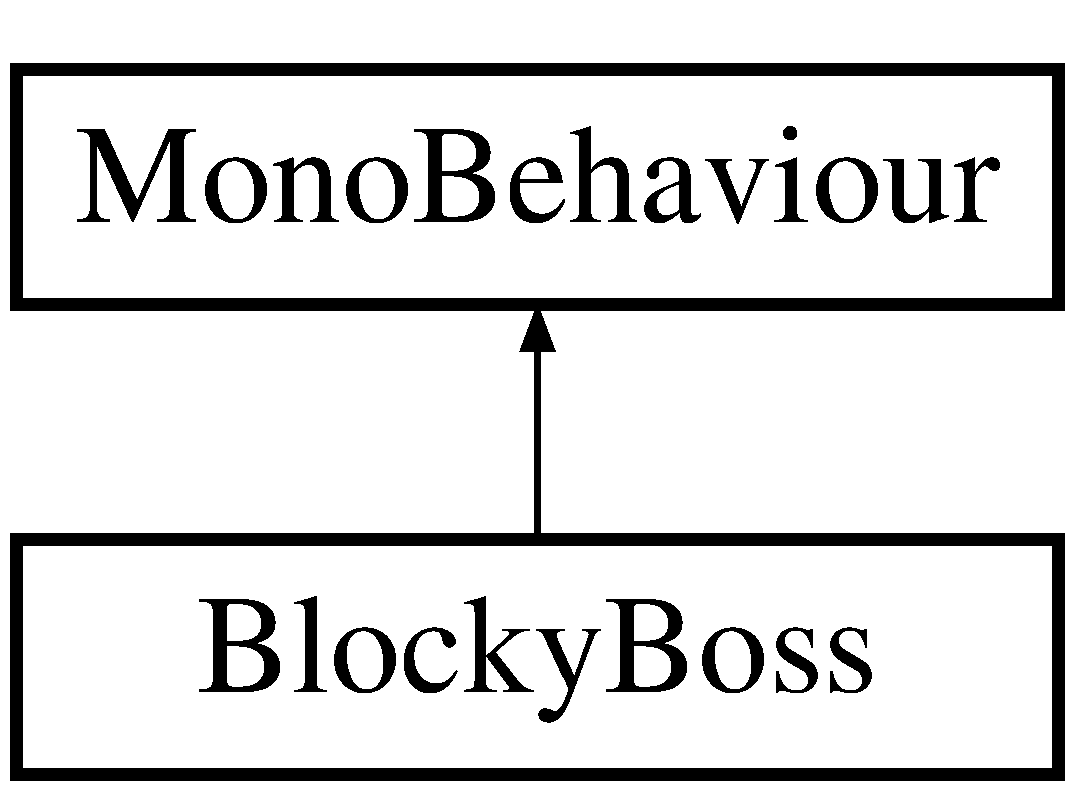
\includegraphics[height=2.000000cm]{class_blocky_boss}
\end{center}
\end{figure}
\subsection*{Public Attributes}
\begin{DoxyCompactItemize}
\item 
\hypertarget{class_blocky_boss_a457e4648d6e2f54cadde4cea73295ead}{}\label{class_blocky_boss_a457e4648d6e2f54cadde4cea73295ead} 
float {\bfseries speed}
\end{DoxyCompactItemize}


The documentation for this class was generated from the following file\+:\begin{DoxyCompactItemize}
\item 
Blocky\+Boss.\+cs\end{DoxyCompactItemize}

\hypertarget{class_camera_control}{}\section{Camera\+Control Class Reference}
\label{class_camera_control}\index{Camera\+Control@{Camera\+Control}}
Inheritance diagram for Camera\+Control\+:\begin{figure}[H]
\begin{center}
\leavevmode
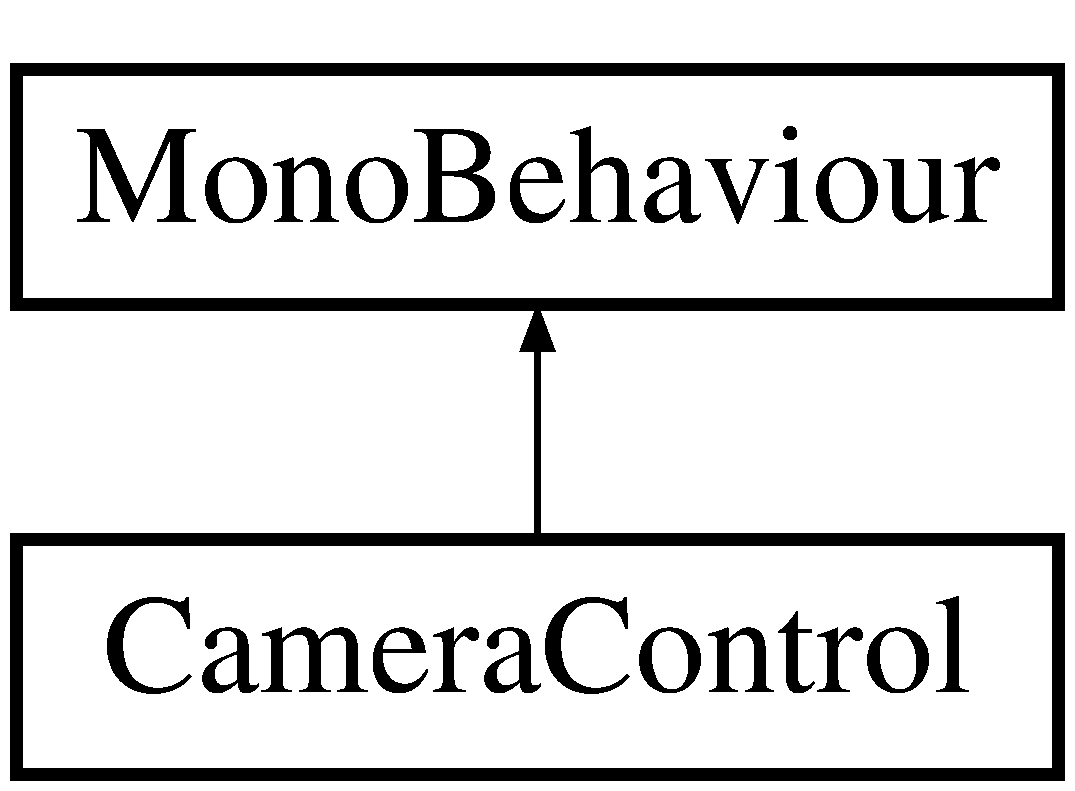
\includegraphics[height=2.000000cm]{class_camera_control}
\end{center}
\end{figure}
\subsection*{Public Attributes}
\begin{DoxyCompactItemize}
\item 
\hypertarget{class_camera_control_a68ca17e97e355b5f391ae4cb11a19680}{}\label{class_camera_control_a68ca17e97e355b5f391ae4cb11a19680} 
Transform {\bfseries target}
\item 
\hypertarget{class_camera_control_a700414c60a426ab8938073d2136974f0}{}\label{class_camera_control_a700414c60a426ab8938073d2136974f0} 
float {\bfseries damping} = 1
\item 
\hypertarget{class_camera_control_a37efa13f7e37cb8ce7e404731605ae17}{}\label{class_camera_control_a37efa13f7e37cb8ce7e404731605ae17} 
float {\bfseries look\+Ahead\+Factor} = 3
\item 
\hypertarget{class_camera_control_acac3aa9575babfcf9e2ccb5aee7f9eb9}{}\label{class_camera_control_acac3aa9575babfcf9e2ccb5aee7f9eb9} 
float {\bfseries look\+Ahead\+Return\+Speed} = 0.\+5f
\item 
\hypertarget{class_camera_control_afe31c94a50cb639ba7bf8fa4815299ff}{}\label{class_camera_control_afe31c94a50cb639ba7bf8fa4815299ff} 
float {\bfseries look\+Ahead\+Move\+Threshold} = 0.\+1f
\end{DoxyCompactItemize}


The documentation for this class was generated from the following file\+:\begin{DoxyCompactItemize}
\item 
Camera\+Control.\+cs\end{DoxyCompactItemize}

\hypertarget{class_camera_follow}{}\section{Camera\+Follow Class Reference}
\label{class_camera_follow}\index{Camera\+Follow@{Camera\+Follow}}
Inheritance diagram for Camera\+Follow\+:\begin{figure}[H]
\begin{center}
\leavevmode
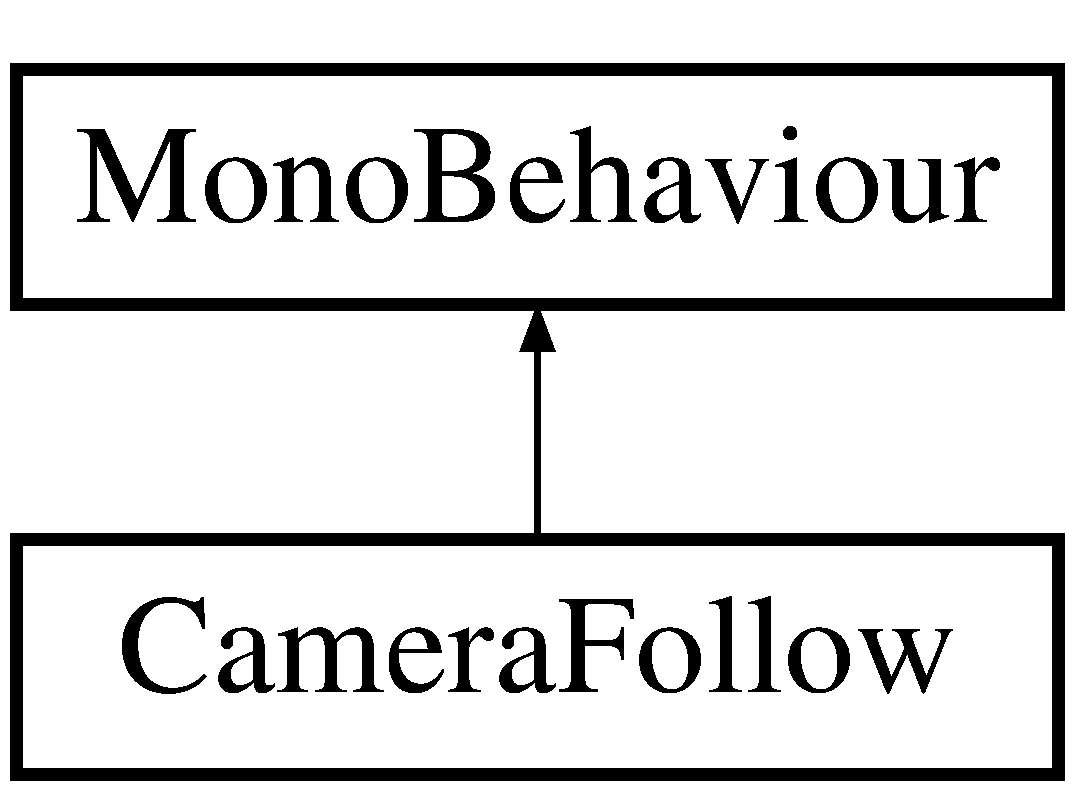
\includegraphics[height=2.000000cm]{class_camera_follow}
\end{center}
\end{figure}
\subsection*{Public Attributes}
\begin{DoxyCompactItemize}
\item 
\hypertarget{class_camera_follow_a81fee88b02e94df331b3f9d2c7cf03b2}{}\label{class_camera_follow_a81fee88b02e94df331b3f9d2c7cf03b2} 
float {\bfseries smooth\+TimeX}
\item 
\hypertarget{class_camera_follow_accdac5d0679acf98fa098f5a8fd7105f}{}\label{class_camera_follow_accdac5d0679acf98fa098f5a8fd7105f} 
float {\bfseries smooth\+TimeY}
\item 
\hypertarget{class_camera_follow_a9d816384fddcc790114d16e5886e051c}{}\label{class_camera_follow_a9d816384fddcc790114d16e5886e051c} 
Game\+Object {\bfseries player}
\item 
\hypertarget{class_camera_follow_add6d71fd83ea10f24ef56ca80e853e9a}{}\label{class_camera_follow_add6d71fd83ea10f24ef56ca80e853e9a} 
bool {\bfseries bounds}
\item 
\hypertarget{class_camera_follow_a0d9dc7c6572cfeffd957e8e63b62969c}{}\label{class_camera_follow_a0d9dc7c6572cfeffd957e8e63b62969c} 
Vector3 {\bfseries min\+Camera\+Pos}
\item 
\hypertarget{class_camera_follow_a6fc27efa09010828e8016e5df83a3c01}{}\label{class_camera_follow_a6fc27efa09010828e8016e5df83a3c01} 
Vector3 {\bfseries max\+Camera\+Pos}
\end{DoxyCompactItemize}


The documentation for this class was generated from the following file\+:\begin{DoxyCompactItemize}
\item 
Camera\+Follow.\+cs\end{DoxyCompactItemize}

\hypertarget{class_character_controller_script}{}\section{Character\+Controller\+Script Class Reference}
\label{class_character_controller_script}\index{Character\+Controller\+Script@{Character\+Controller\+Script}}
Inheritance diagram for Character\+Controller\+Script\+:\begin{figure}[H]
\begin{center}
\leavevmode
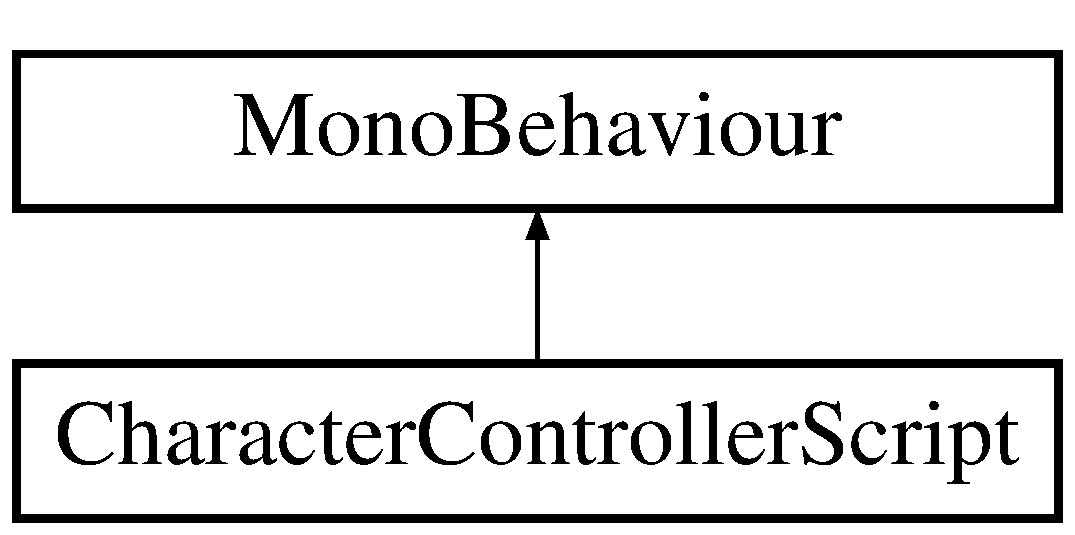
\includegraphics[height=2.000000cm]{class_character_controller_script}
\end{center}
\end{figure}
\subsection*{Public Attributes}
\begin{DoxyCompactItemize}
\item 
\hypertarget{class_character_controller_script_ab0158aad94e83ea978139fc8e3946b5a}{}\label{class_character_controller_script_ab0158aad94e83ea978139fc8e3946b5a} 
float {\bfseries max\+Speed} = 10f
\item 
\hypertarget{class_character_controller_script_a7d59fd6ab8ee7ab3b91206457bbd19f7}{}\label{class_character_controller_script_a7d59fd6ab8ee7ab3b91206457bbd19f7} 
float {\bfseries jump\+Force} = 700f
\item 
\hypertarget{class_character_controller_script_a7f84311277b867c89b5e3a8b640d6a44}{}\label{class_character_controller_script_a7f84311277b867c89b5e3a8b640d6a44} 
Transform {\bfseries ground\+Check}
\item 
\hypertarget{class_character_controller_script_a5d0d8ebbb1d5c74bde4ada1b14e88ced}{}\label{class_character_controller_script_a5d0d8ebbb1d5c74bde4ada1b14e88ced} 
Layer\+Mask {\bfseries what\+Is\+Ground}
\item 
\hypertarget{class_character_controller_script_ae05fea6fa89d070f3897f6038bf0407f}{}\label{class_character_controller_script_ae05fea6fa89d070f3897f6038bf0407f} 
bool {\bfseries jump} = false
\item 
\hypertarget{class_character_controller_script_ae9027bd9082b11140a70691a44202d10}{}\label{class_character_controller_script_ae9027bd9082b11140a70691a44202d10} 
string {\bfseries message} = \char`\"{}Power Up\+: Jumping acquired.\char`\"{}
\item 
\hypertarget{class_character_controller_script_a5a902e98061e6f9656cf0e7deb42b439}{}\label{class_character_controller_script_a5a902e98061e6f9656cf0e7deb42b439} 
float {\bfseries display\+Time}
\item 
\hypertarget{class_character_controller_script_ad5e60344614af133fa68c6b5e8b50192}{}\label{class_character_controller_script_ad5e60344614af133fa68c6b5e8b50192} 
bool {\bfseries display\+Message} = false
\end{DoxyCompactItemize}


The documentation for this class was generated from the following file\+:\begin{DoxyCompactItemize}
\item 
Character\+Controller\+Script.\+cs\end{DoxyCompactItemize}

\hypertarget{class_destroy_floor5}{}\section{Destroy\+Floor5 Class Reference}
\label{class_destroy_floor5}\index{Destroy\+Floor5@{Destroy\+Floor5}}
Inheritance diagram for Destroy\+Floor5\+:\begin{figure}[H]
\begin{center}
\leavevmode
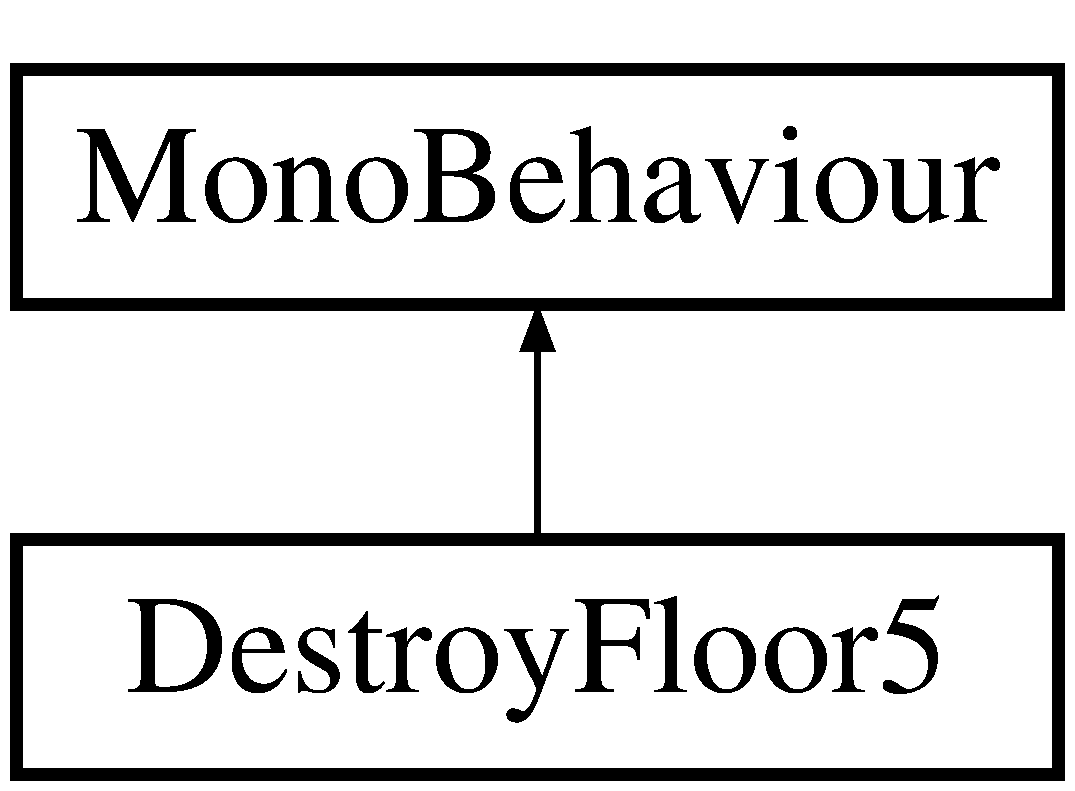
\includegraphics[height=2.000000cm]{class_destroy_floor5}
\end{center}
\end{figure}


The documentation for this class was generated from the following file\+:\begin{DoxyCompactItemize}
\item 
Destroy\+Floor5.\+cs\end{DoxyCompactItemize}

\hypertarget{class_enemies_chase}{}\section{Enemies\+Chase Class Reference}
\label{class_enemies_chase}\index{Enemies\+Chase@{Enemies\+Chase}}
Inheritance diagram for Enemies\+Chase\+:\begin{figure}[H]
\begin{center}
\leavevmode
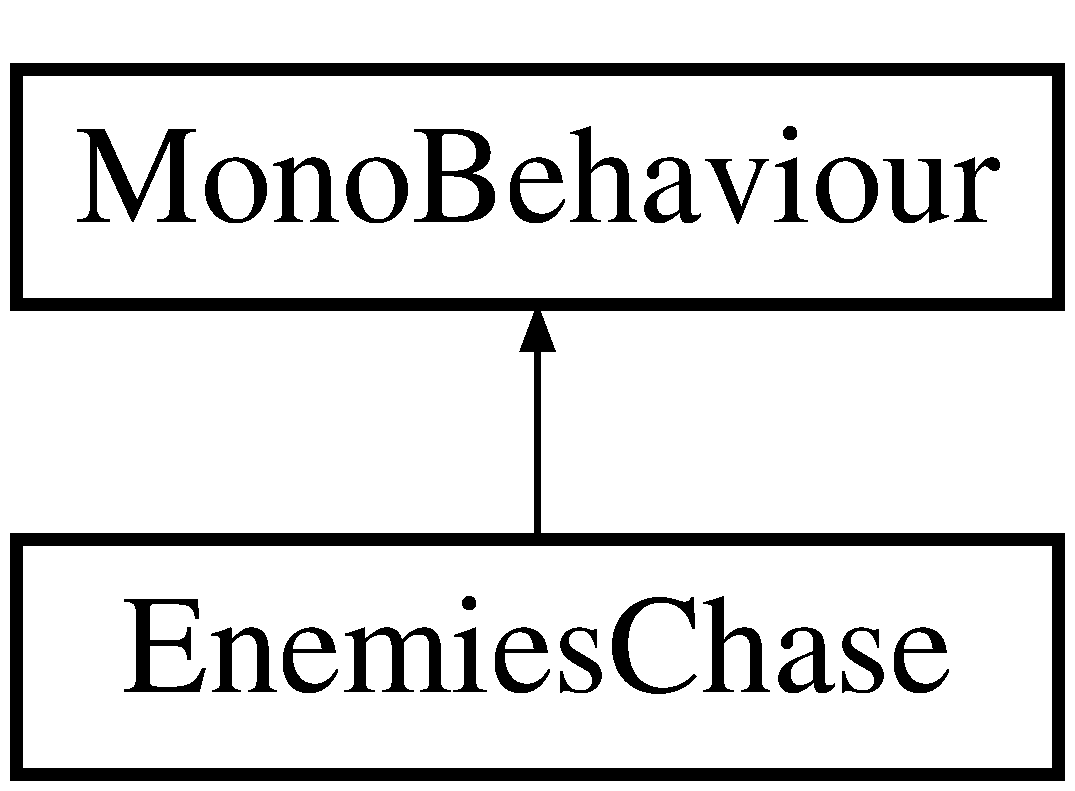
\includegraphics[height=2.000000cm]{class_enemies_chase}
\end{center}
\end{figure}
\subsection*{Public Attributes}
\begin{DoxyCompactItemize}
\item 
\hypertarget{class_enemies_chase_a00dbfcc4c86b3d505e4119d687423d9e}{}\label{class_enemies_chase_a00dbfcc4c86b3d505e4119d687423d9e} 
float {\bfseries speed}
\item 
\hypertarget{class_enemies_chase_a9fd0c00922f4bd8dc44c67c972a9c0e3}{}\label{class_enemies_chase_a9fd0c00922f4bd8dc44c67c972a9c0e3} 
Game\+Object {\bfseries player}
\item 
\hypertarget{class_enemies_chase_a2c390ef44b3c3be24ee5b2ffaa083a2d}{}\label{class_enemies_chase_a2c390ef44b3c3be24ee5b2ffaa083a2d} 
Game\+Object {\bfseries enemy}
\end{DoxyCompactItemize}


The documentation for this class was generated from the following file\+:\begin{DoxyCompactItemize}
\item 
Enemies\+Chase.\+cs\end{DoxyCompactItemize}

\hypertarget{class_enemies_on_floor2}{}\section{Enemies\+On\+Floor2 Class Reference}
\label{class_enemies_on_floor2}\index{Enemies\+On\+Floor2@{Enemies\+On\+Floor2}}
Inheritance diagram for Enemies\+On\+Floor2\+:\begin{figure}[H]
\begin{center}
\leavevmode
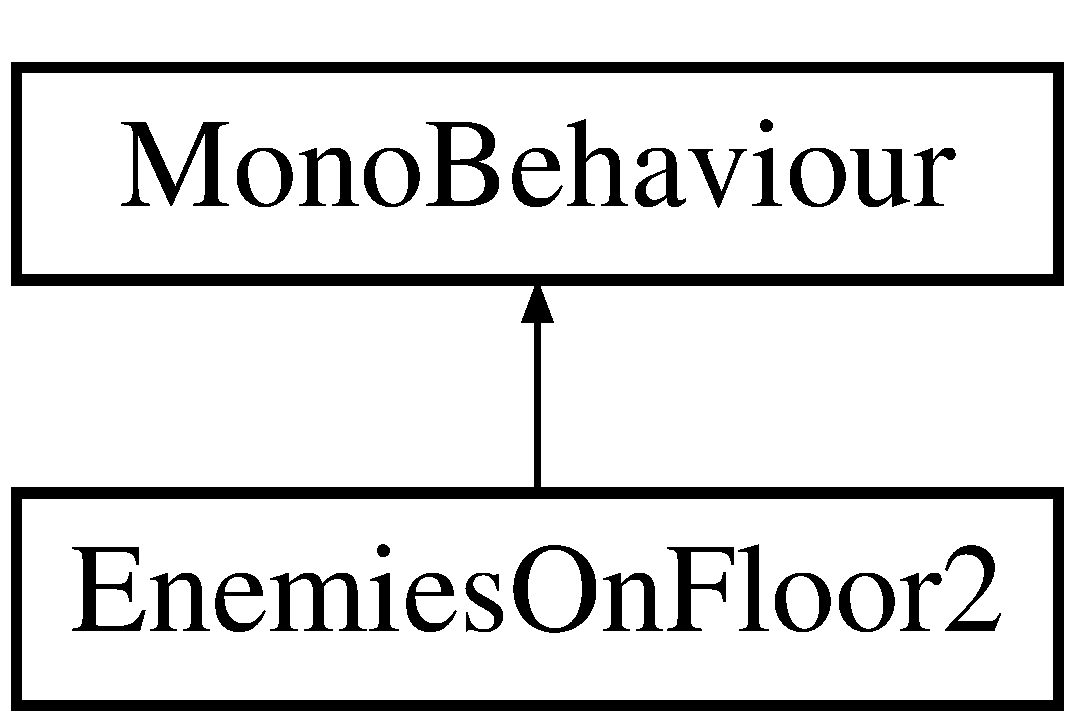
\includegraphics[height=2.000000cm]{class_enemies_on_floor2}
\end{center}
\end{figure}


The documentation for this class was generated from the following file\+:\begin{DoxyCompactItemize}
\item 
Enemies\+On\+Floor2.\+cs\end{DoxyCompactItemize}

\hypertarget{class_enemies_on_floor3}{}\section{Enemies\+On\+Floor3 Class Reference}
\label{class_enemies_on_floor3}\index{Enemies\+On\+Floor3@{Enemies\+On\+Floor3}}
Inheritance diagram for Enemies\+On\+Floor3\+:\begin{figure}[H]
\begin{center}
\leavevmode
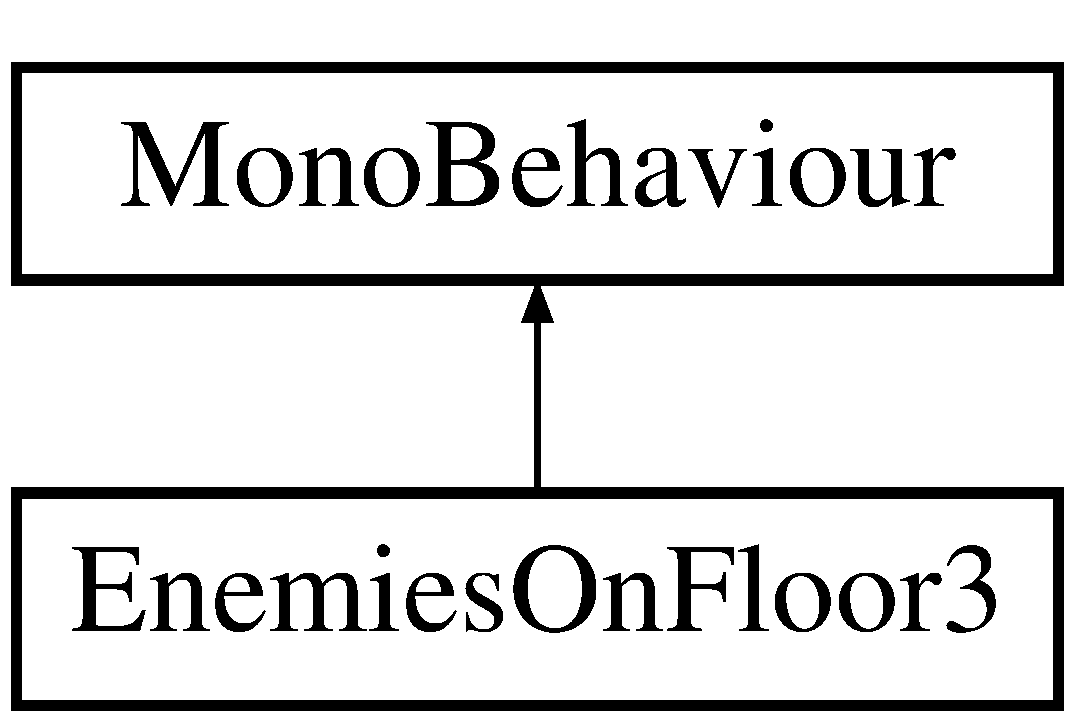
\includegraphics[height=2.000000cm]{class_enemies_on_floor3}
\end{center}
\end{figure}


The documentation for this class was generated from the following file\+:\begin{DoxyCompactItemize}
\item 
Enemies\+On\+Floor3.\+cs\end{DoxyCompactItemize}

\hypertarget{class_enemies_on_floor4}{}\section{Enemies\+On\+Floor4 Class Reference}
\label{class_enemies_on_floor4}\index{Enemies\+On\+Floor4@{Enemies\+On\+Floor4}}
Inheritance diagram for Enemies\+On\+Floor4\+:\begin{figure}[H]
\begin{center}
\leavevmode
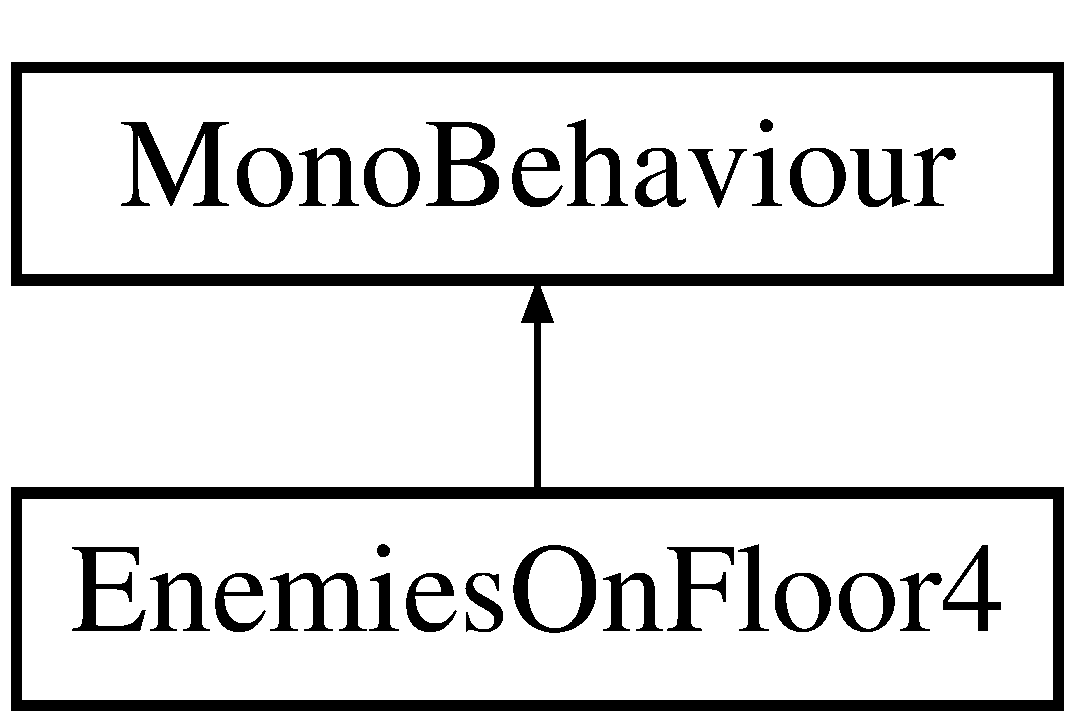
\includegraphics[height=2.000000cm]{class_enemies_on_floor4}
\end{center}
\end{figure}


The documentation for this class was generated from the following file\+:\begin{DoxyCompactItemize}
\item 
Enemies\+On\+Floor4.\+cs\end{DoxyCompactItemize}

\hypertarget{class_enemy_script}{}\section{Enemy\+Script Class Reference}
\label{class_enemy_script}\index{Enemy\+Script@{Enemy\+Script}}
Inheritance diagram for Enemy\+Script\+:\begin{figure}[H]
\begin{center}
\leavevmode
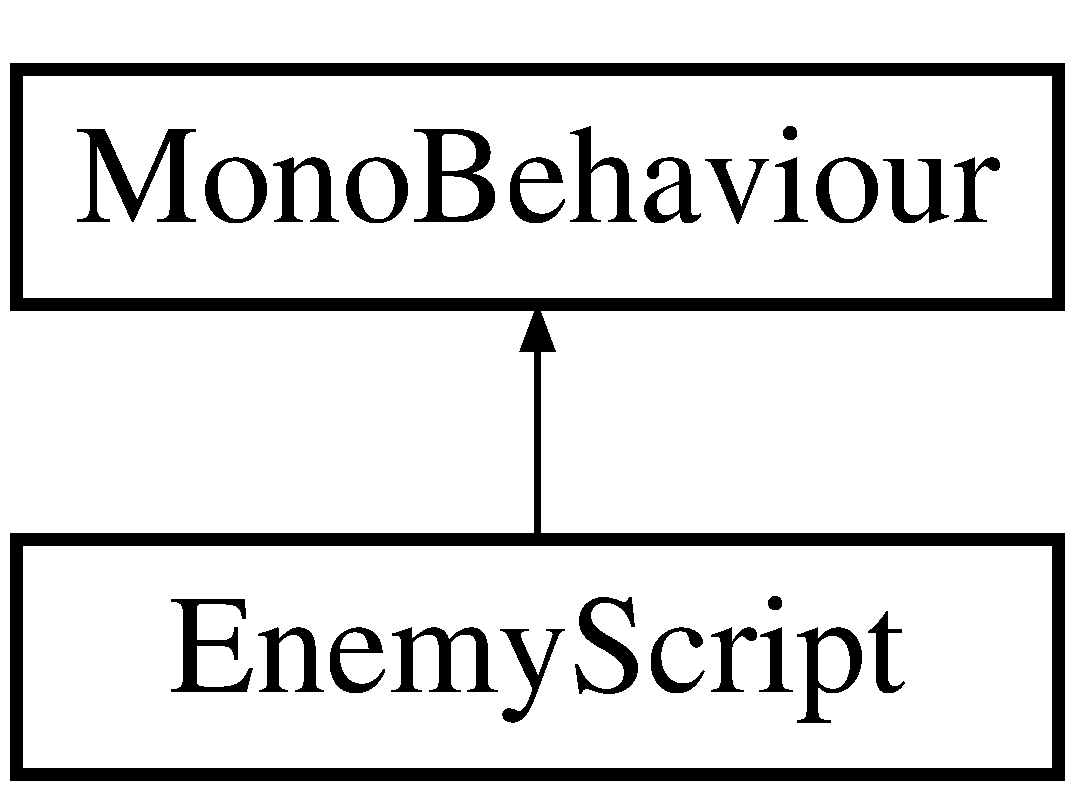
\includegraphics[height=2.000000cm]{class_enemy_script}
\end{center}
\end{figure}
\subsection*{Public Attributes}
\begin{DoxyCompactItemize}
\item 
\hypertarget{class_enemy_script_a2c618fda4a3b98cd7fc1089c682c3e90}{}\label{class_enemy_script_a2c618fda4a3b98cd7fc1089c682c3e90} 
float {\bfseries speed}
\end{DoxyCompactItemize}


The documentation for this class was generated from the following file\+:\begin{DoxyCompactItemize}
\item 
Enemy\+Script.\+cs\end{DoxyCompactItemize}

\hypertarget{class_mega_jump_pow_up}{}\section{Mega\+Jump\+Pow\+Up Class Reference}
\label{class_mega_jump_pow_up}\index{Mega\+Jump\+Pow\+Up@{Mega\+Jump\+Pow\+Up}}
Inheritance diagram for Mega\+Jump\+Pow\+Up\+:\begin{figure}[H]
\begin{center}
\leavevmode
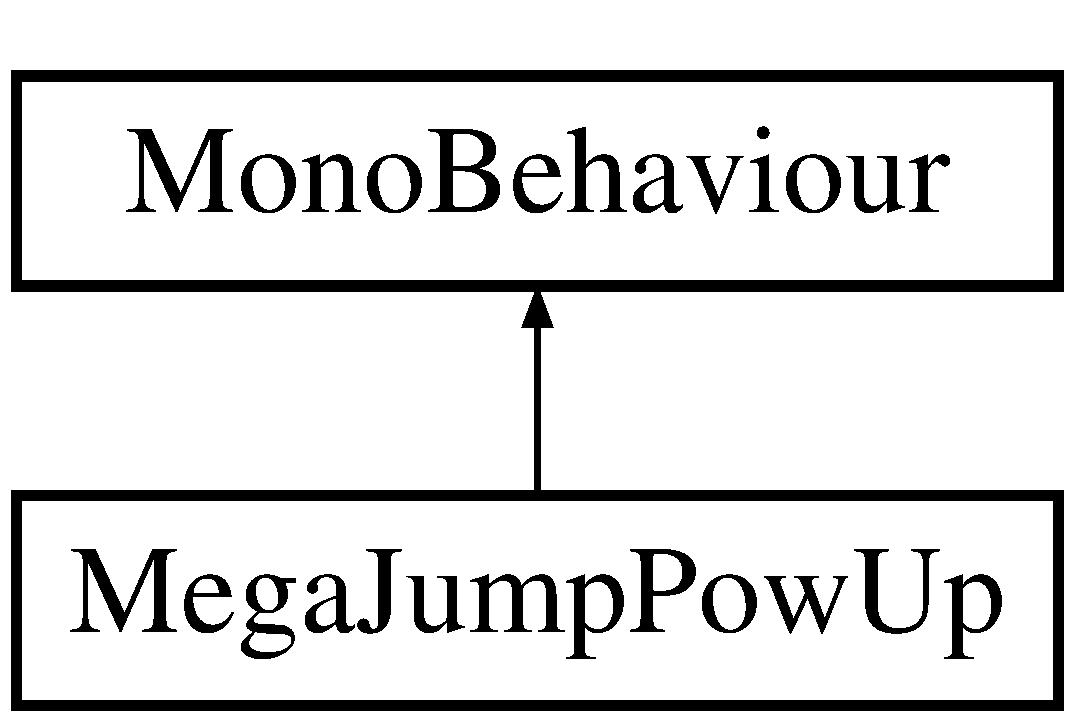
\includegraphics[height=2.000000cm]{class_mega_jump_pow_up}
\end{center}
\end{figure}


The documentation for this class was generated from the following file\+:\begin{DoxyCompactItemize}
\item 
Mega\+Jump\+Pow\+Up.\+cs\end{DoxyCompactItemize}

\hypertarget{class_on_floor5}{}\section{On\+Floor5 Class Reference}
\label{class_on_floor5}\index{On\+Floor5@{On\+Floor5}}
Inheritance diagram for On\+Floor5\+:\begin{figure}[H]
\begin{center}
\leavevmode
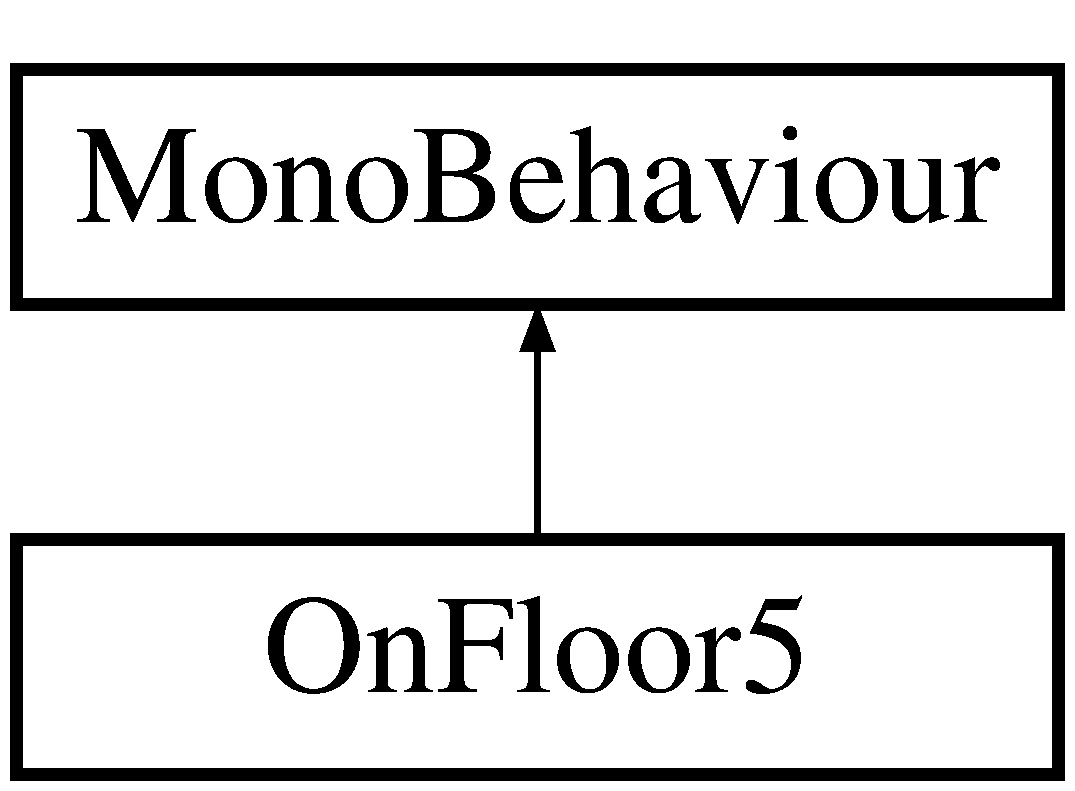
\includegraphics[height=2.000000cm]{class_on_floor5}
\end{center}
\end{figure}
\subsection*{Public Attributes}
\begin{DoxyCompactItemize}
\item 
\hypertarget{class_on_floor5_a9e6c5a8af8502f16a41500d4dd60ba01}{}\label{class_on_floor5_a9e6c5a8af8502f16a41500d4dd60ba01} 
float {\bfseries display\+Time}
\item 
\hypertarget{class_on_floor5_ad33d555a7c4f5db4aad2ef16dc565683}{}\label{class_on_floor5_ad33d555a7c4f5db4aad2ef16dc565683} 
bool {\bfseries display\+Message} = false
\end{DoxyCompactItemize}


The documentation for this class was generated from the following file\+:\begin{DoxyCompactItemize}
\item 
On\+Floor5.\+cs\end{DoxyCompactItemize}

\hypertarget{class_powerups}{}\section{Powerups Class Reference}
\label{class_powerups}\index{Powerups@{Powerups}}
Inheritance diagram for Powerups\+:\begin{figure}[H]
\begin{center}
\leavevmode
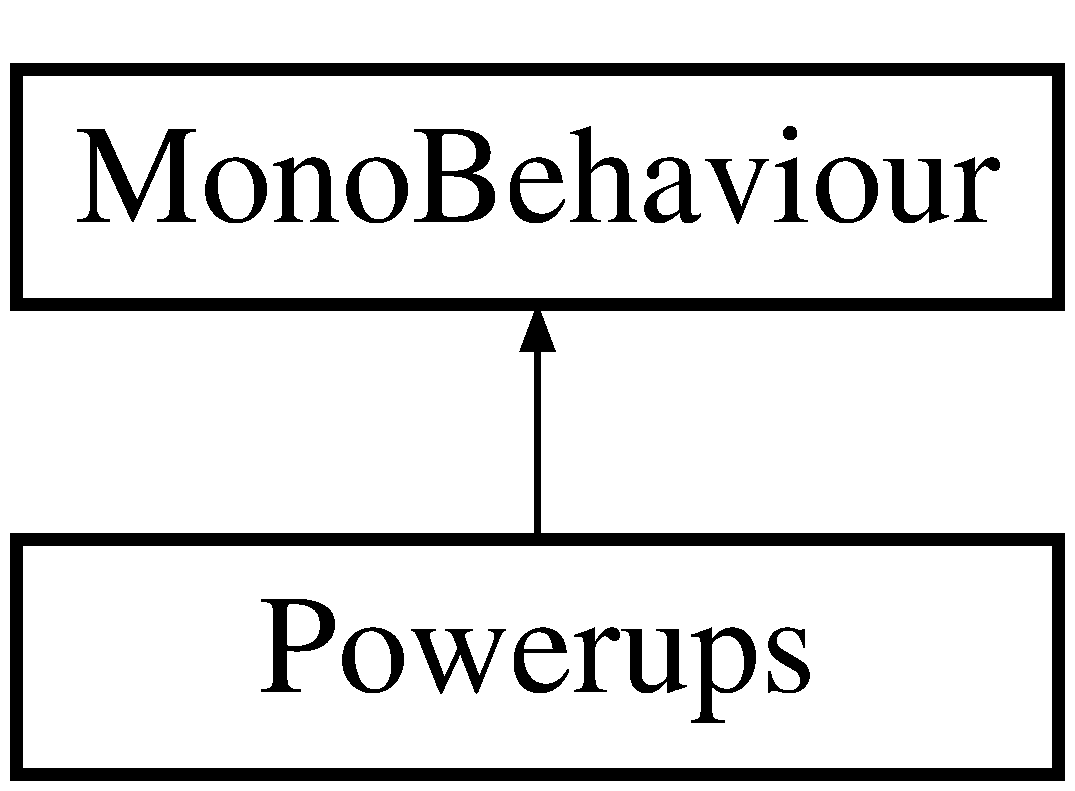
\includegraphics[height=2.000000cm]{class_powerups}
\end{center}
\end{figure}


The documentation for this class was generated from the following file\+:\begin{DoxyCompactItemize}
\item 
Powerups.\+cs\end{DoxyCompactItemize}

\hypertarget{class_repeat_sprite_boundary}{}\section{Repeat\+Sprite\+Boundary Class Reference}
\label{class_repeat_sprite_boundary}\index{Repeat\+Sprite\+Boundary@{Repeat\+Sprite\+Boundary}}
Inheritance diagram for Repeat\+Sprite\+Boundary\+:\begin{figure}[H]
\begin{center}
\leavevmode
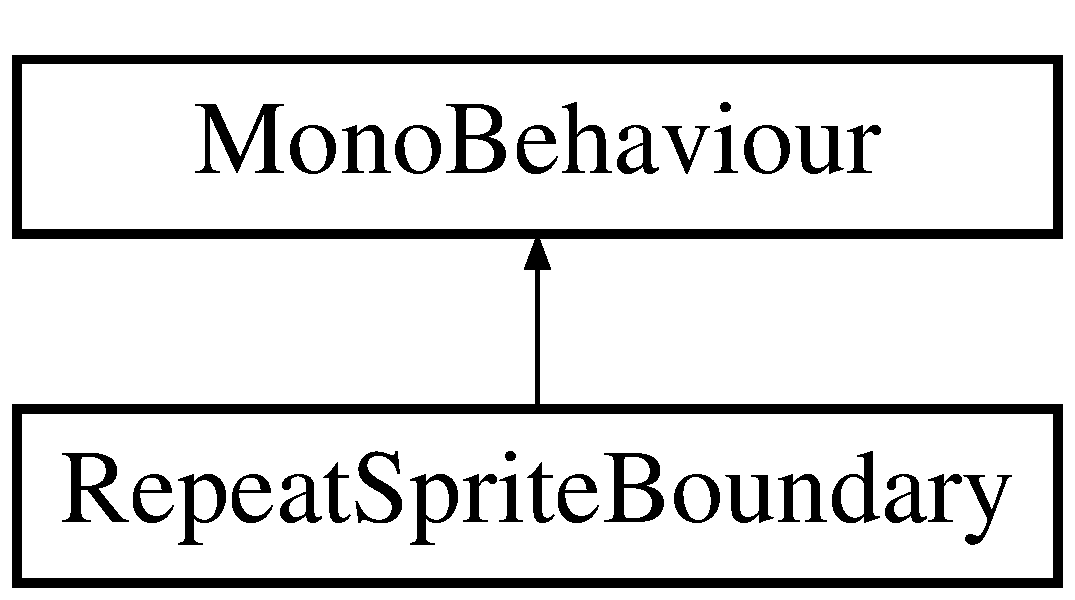
\includegraphics[height=2.000000cm]{class_repeat_sprite_boundary}
\end{center}
\end{figure}


The documentation for this class was generated from the following file\+:\begin{DoxyCompactItemize}
\item 
Repeat\+Sprite\+Boundary.\+cs\end{DoxyCompactItemize}

\hypertarget{class_restart_game}{}\section{Restart\+Game Class Reference}
\label{class_restart_game}\index{Restart\+Game@{Restart\+Game}}
Inheritance diagram for Restart\+Game\+:\begin{figure}[H]
\begin{center}
\leavevmode
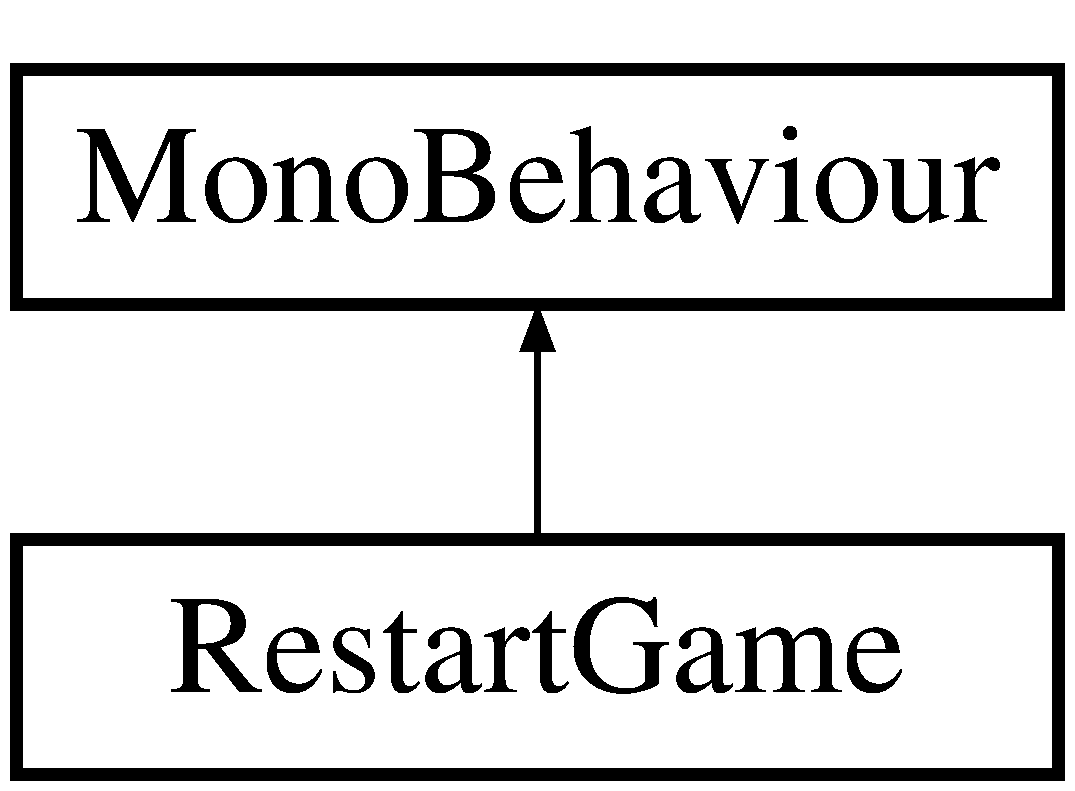
\includegraphics[height=2.000000cm]{class_restart_game}
\end{center}
\end{figure}


The documentation for this class was generated from the following file\+:\begin{DoxyCompactItemize}
\item 
Restart\+Game.\+cs\end{DoxyCompactItemize}

\hypertarget{class_scene_switch}{}\section{Scene\+Switch Class Reference}
\label{class_scene_switch}\index{Scene\+Switch@{Scene\+Switch}}
Inheritance diagram for Scene\+Switch\+:\begin{figure}[H]
\begin{center}
\leavevmode
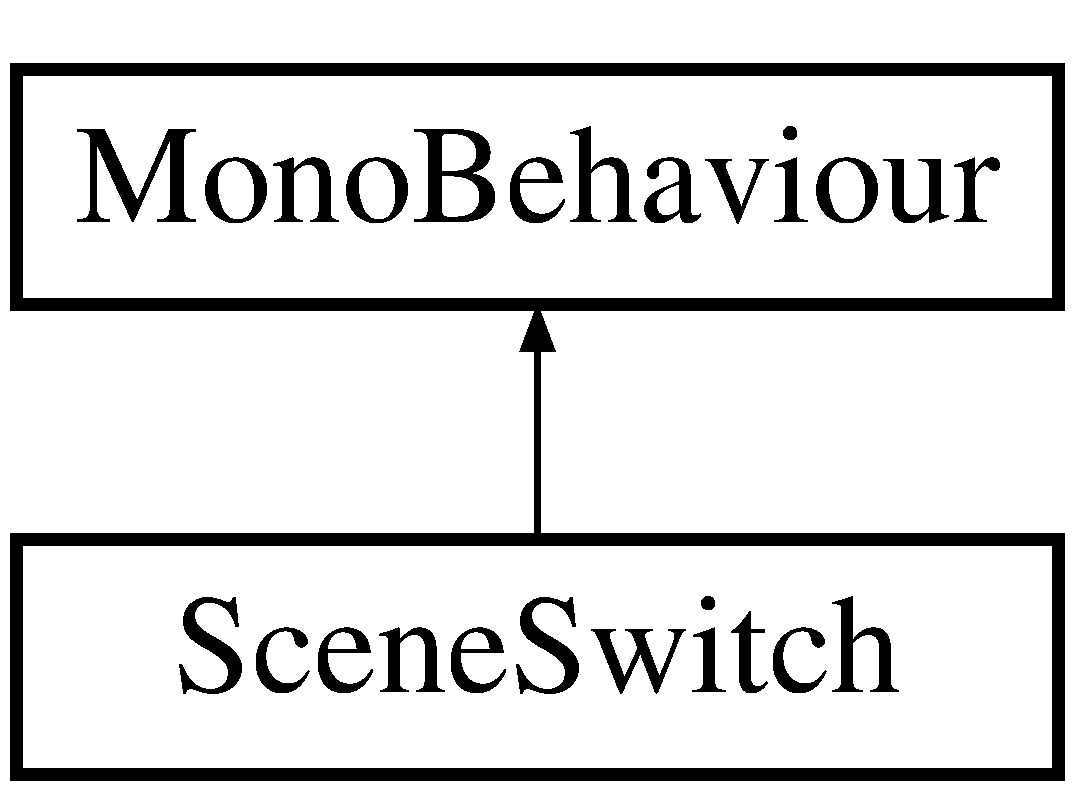
\includegraphics[height=2.000000cm]{class_scene_switch}
\end{center}
\end{figure}
\subsection*{Public Types}
\begin{DoxyCompactItemize}
\item 
\hypertarget{class_scene_switch_ace7e42686aab3de3d3e557cfda84619a}{}\label{class_scene_switch_ace7e42686aab3de3d3e557cfda84619a} 
enum {\bfseries Stages} \{ {\bfseries S\+T\+A\+G\+E1}, 
{\bfseries S\+C\+E\+N\+E\+D\+E\+N\+AE}, 
{\bfseries S\+T\+A\+G\+E\+L1}, 
{\bfseries S\+T\+A\+G\+E\+L2}
 \}
\end{DoxyCompactItemize}
\subsection*{Public Attributes}
\begin{DoxyCompactItemize}
\item 
\hypertarget{class_scene_switch_a4c670b4004c0e5259675872144f9dc6c}{}\label{class_scene_switch_a4c670b4004c0e5259675872144f9dc6c} 
Stages {\bfseries my\+Stage}
\end{DoxyCompactItemize}


The documentation for this class was generated from the following file\+:\begin{DoxyCompactItemize}
\item 
Scene\+Switch.\+cs\end{DoxyCompactItemize}

%--- End generated contents ---

% Index
\backmatter
\newpage
\phantomsection
\clearemptydoublepage
\addcontentsline{toc}{chapter}{Index}
\printindex

\end{document}
